%! Author = Charles Yang

% Preamble
\documentclass[11pt]{article}

% Packages
\usepackage{amsmath}
\usepackage{amsfonts}
\usepackage{hyperref}
\usepackage{enumitem}
\usepackage{graphicx}

% Settings
\setlist[enumerate]{font=\bfseries}

% Title Info
\title{STAT 347 HW5}
\author{Charles Yang}

\addtolength{\oddsidemargin}{-.875in}
\addtolength{\evensidemargin}{-.875in}
\addtolength{\textwidth}{1.75in}
\addtolength{\topmargin}{-.875in}
\addtolength{\textheight}{1.75in}

% Document
\begin{document}
    \maketitle

    \begin{enumerate}

        \item[3.105]
        \begin{enumerate}
            \item[a] Y has a hypergeometric distribution because we are selecting candidates without replacement.
            \item[b] $P(Y \geq 2) = P(2) + P(3) = \frac{C(5, 2)C(3, 1)}{C(8, 3)} + \frac{C(5, 3)C(3, 0)}{C(8, 3)}$
            \item[c] $E(Y) = (3*5)/8 = 1.875$, $V(Y) = 8 \frac{5}{8} \frac{3}{8} \frac{5}{7} = 0.502$
        \end{enumerate}

        \item[3.106] $E(X) = 5*4/10 = 2$. $2 * 50 = 100$ \\
                     $V(50X) = 50^2 V(X) = 2500 * 5 * (4/10) * (10-4)/10 * (10 - 5)/(10 - 1) = 1667$

        \item[3.121]
        \begin{enumerate}
            \item[a] $P(Y = 4) = \frac{2^4*e^{-2}}{4!} = 0.9$
            \item[b] $P(Y \geq 4) = 1 - \sum_{i = 0}^3 \frac{2^i*e^{-2}}{i!} = 0.143$
            \item[c] $P(Y < 4) = 1 - P(Y \geq 4) = 0.857$
            \item[d] $P(Y \geq 4 | Y \geq 2) = \frac{P(Y \geq 4 \;\&\; Y \geq 2)}{P(Y \geq 2)} = \frac{P(Y \geq 4)}{1 - P(Y < 2)}$ \\
                     $= \frac{0.143}{1 - P(0) - P(1)} = 0.241$
        \end{enumerate}

        \item[3.122]
        \begin{enumerate}
            \item[a] $P(Y \leq 3) = \sum_{i = 0}^3 \frac{7^i*e^{-7}}{i!} = 0.082$
            \item[b] $P(Y \geq 2) = 1 - P(0) - P(1) = 0.993$
            \item[c] $P(Y = 5) = \frac{7^5}{e^7*5!} = 0.128$
        \end{enumerate}

        \item[3.132] This is reasonable because we know the average given a certain time period, \\
                    and we want to calculate probability of a value during that time period. \\
                    A Poisson distribution is reasonable here. \\
                    $P(Y > 3) = 1 - \sum_{i = 0}^3 \frac{1^i*e^{-1}}{i!} = 1 - \sum_{i = 0}^3 \frac{1}{e*i!} = 0.019$

        \item[3.147] Geometric moment generating function
        \begin{align*}
            m_y(t) &= E(e^{ty}) \text{, and } P(y) = q^{y - 1} p \\
            &= \sum_{y=1}^{\infty} e^{ty}q^{y - 1} p \\
            &= \sum_{y=1}^{\infty} e^{ty}q^y q^{-1} p \\
            &= \frac{p}{q} \sum_{y=1}^{\infty} e^{ty}q^y \\
            &= \frac{p}{q} \sum_{y=1}^{\infty} (e^{t}q)^y \\
            &= \frac{p}{q} \frac{qe^t}{1 - qe^t} \\
            &= \frac{pe^t}{1 - qe^t}
        \end{align*}

        \item[3.148]
        \begin{align*}
            E(Y) &= \frac{d}{dt} [\frac{pe^t}{1 - qe^t}] \\
            &= p \frac{(1-qe^t)*e^t + e^t(qe^t)}{(1 - qe^t)^2} \\
            &= pe^t \frac{(1-qe^t) + (qe^t)}{(1 - qe^t)^2} \\
            &= \frac{pe^t}{(1 - qe^t)^2} \\
            &= \frac{p}{(1 - (1 - p))^2} \text{ at } t = 0 \\
            &= \frac{p}{p^2} = \frac{1}{p}
        \end{align*}
        \begin{align*}
            E(Y^2) &= (\frac{pe^t}{(1 - qe^t)^2})' \\
            &= p \frac{(1 - qe^t)^2 e^t + 2e^t (1-qe^t)qe^t}{(1-qe^t)^4} \\
            &= pe^t \frac{(1 - qe^t)^2 + 2 (1-qe^t)qe^t}{(1-qe^t)^4} \\
            &= pe^t \frac{1 - qe^t + 2qe^t}{(1-qe^t)^3} \\
            &= pe^t \frac{1 + qe^t}{(1-qe^t)^3} \\
            &= p \frac{1 + q}{(1-q)^3} \text{ at } t = 0 \\
            &= \frac{2 - p}{p^2} \\ \\
            V(Y) = E(Y^2) - E(Y)^2 &= \frac{2 - p}{p^2} - \frac{1}{p^2} = \frac{1 - p}{p^2}
        \end{align*}

        \item[3.158] $E(e^{aY+b}) = E(e^{bt} e^{atY}) = e^{bt} E(e^{atY}) = e^{bt} m(at)$

        \item[3.167]
        \begin{enumerate}
            \item[a] $P(6 - 11 < Y - \mu < 16 - 11) = P(|Y - \mu| < 5) \geq 1 - \frac{3^2}{5^2} = 16/25$
            \item[b]
            \begin{align*}
                1 - P(|Y - 11| < C) \leq 0.09 \\
                P(|Y - 11| < C) \geq 0.91 \\
                P(-C < Y - 11 < C) \geq 0.91 \\
                P(11 - C < Y - 11 < 11 + C) \geq 0.91 \\
                1 - \frac{1}{k^2} = 0.91 \implies k = 10/3 \\
                C = k \sigma = 3*10/3 = 10
            \end{align*}
        \end{enumerate}

        \item[4.1]
         \[
             F(y) = \begin{cases}
                0 & -\infty < y < 1 \\
                0.3 & 1 \leq y < 2 \\
                0.7 & 2 \leq y < 3 \\
                0.9 & 3 \leq y < 4 \\
                1 & 4 \leq y < \infty
            \end{cases}
        \]
        \\
        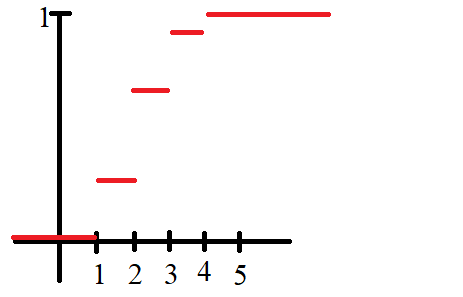
\includegraphics{4.1b.png}

        \item[4.18]
        \begin{enumerate}
            \item[a]
            \begin{align*}
                \int_{-1}^0 0.2 dy + \int_0^1 0.2 + cy dy = 1 \\
                0.2y |_{-1}^0 + (0.2y + \frac{cy^2}{2}) |_0^1 = 1 \\
                0.2 + 0.2 + \frac{c}{2} = 1 \\
                \frac{c}{2} = 0.6 \\
                c = 1.2
            \end{align*}
            \item[b] Integrals done on paper... $F(y) = \int_{-\infty}^y f(t) dt$
            \[
                F(y) = \begin{cases}
                           0 & y \leq -1 \\
                           0.2+0.2y & -1 < y \leq 0 \\
                           0.6y^2 + 0.2y + 0.2 & 0 < y \leq 1 \\
                           1 & y > 1
                \end{cases}
            \]
            \item[c]
            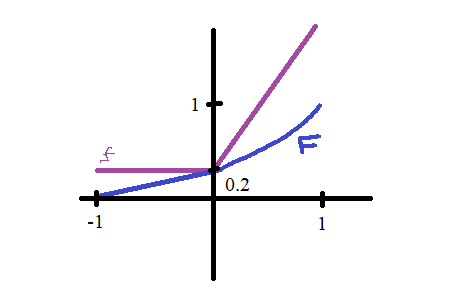
\includegraphics{4.18c.png}
            \item[d] $F(-1) = 0$, $F(0) = 0.2$, $F(1) = 0.6 + 0.2 + 0.2 = 1$
            \item[e] $\int_0^{1/2} 0.2 + 0.2y dy = 0.25$
            \item[f]
            \begin{align*}
                \frac{P(Y > 0.5 \;\&\; P > 0.1)}{P(Y > 0.1)} &= \frac{P(Y > 0.5)}{P(Y > 0.1)} \\
                &= \frac{1 - P(Y \leq 0.5)}{1 - P(Y \leq 0.1)} \\
                &= \frac{1 - F(0.5)}{1 - F(0.1)} \\
                &= 0.7106
            \end{align*}
        \end{enumerate}

        \item[4.22] $\int_{-1}^0 0.2y dy + \int_0^1 0.2y+1.2y^2 dy = -0.1 + 0.7 = 0.6$ \\
                    $\int_{-1}^0 0.2y^2 dy + \int_0^1 0.2y^2+1.2y^3 dy = 0.2/3 + 0.2/3 + 0.3 = 0.43333$ \\
                    $V(Y) = 0.43333333333 - (0.6)^2 = 0.07333333333$

        \item[4.22]
        \begin{align*}
            E(Y) &= \int_0^1 \frac{3}{2}y^3 + y^2 \\
            &= \frac{3y^4}{8} + \frac{y^3}{3} |_0^1 \\
            &= \frac{3}{8} + \frac{1}{3} = 17/24 \\
            E(Y^2) &= \int_0^1 \frac{3}{2}y^4 + y^3 \\
            &= \frac{3y^5}{10} + \frac{y^4}{4} |_0^1 \\
            &= 3/10 + 1/4 = 11/20 \\
            E(5 - \frac{Y}{2}) &= 5 - \frac{E(Y)}{2} = 4.646 \\
            V(Y) &= 11/20 - (17/24)^2 = 0.0483 \\
            V(5 - \frac{Y}{2}) &= 0.0483*(-0.5)^2 = 0.012
        \end{align*}

    \end{enumerate}

\end{document}